\documentclass[12pt]{article}
\usepackage[utf8]{inputenc}
\usepackage[brazil]{babel}
\usepackage{graphicx}
\usepackage{geometry}
\usepackage{adjustbox}
\usepackage{booktabs}
\usepackage{setspace}
\geometry{a4paper, margin=1in}
\usepackage[hyphens]{url}
\usepackage[hidelinks]{hyperref}  
\usepackage{float}

\begin{document}

\begin{center}
\textbf{RELATÓRIO TÉCNICO}
\end{center}

\noindent\textbf{DISCIPLINA:} Estatística e Probabilidade \\
\noindent\textbf{TURMA:} 4º B \\
\noindent\textbf{ALUNOS:} Thiago Queiroz e Julia Sales \\
\noindent\textbf{PROFESSOR:} Guilherme \\
\noindent\textbf{TEMA:} Análise Estatística do Impacto Global das IAs  \\

\doublespacing

\section*{1. INTRODUÇÃO}

Este relatório tem como objetivo aplicar conceitos fundamentais de Estatística e Probabilidade na análise do \textbf{Global AI Content Impact Dataset}, que se trata de um dataset que contempla métricas de impacto de conteúdo gerado por Inteligência Artificial ao redor do mundo, dividido por país, tipo de mídia, engajamento, confiança e outros fatores.

A análise aqui apresentada aborda estatística descritiva, normalização de dados, distribuições amostrais, cálculo de intervalos de confiança, bem como visualizações gráficas relevantes, permitindo uma visão crítica do fenômeno de IA aplicada à produção de conteúdo em escala global.

O tema chama atenção devido a sua relevância, pois a IA generativa, como modelos de texto, imagem e vídeo, está transformando, de forma permanente, setores como educação, mídia, política e mercado de trabalho. Avaliar seu impacto de forma estatística é fundamental para compreender os padrões relacionado e apoiar a formulação de políticas públicas e estratégias corporativas.

\section*{2. METODOLOGIA}

A base de dados foi processada e analisada no ambiente Google Colab utilizando Python com as bibliotecas \texttt{pandas}, \texttt{numpy}, \texttt{seaborn} e \texttt{matplotlib}. Foram realizadas as seguintes etapas:

\begin{itemize}
    \item Leitura do conjunto de dados.
    \item  Análise estatística descritiva das variáveis quantitativas e a geração de gráficos exploratórios (boxplots, histogramas, dispersão e mapa de calor).
    \item Normalização padrão (z-score) de variáveis selecionadas.
    \item Construção de distribuições amostrais das médias.
    \item Cálculo de intervalos de confiança 
\end{itemize}

\section*{3. DESENVOLVIMENTO}

\subsection*{3.1 Estatística Descritiva}

As seguintes variáveis quantitativas foram analisadas nos gráficos de Boxplots, Histogramas e Mapa de Calor:
\textit{AI Adoption Rate (\%)}, \textit{Job Loss Due to AI (\%)}, \textit{Revenue Increase Due to AI (\%)}, \textit{AI-Generated Content Volume (TBs per year)}, \textit{Human-AI Collaboration Rate (\%)} e \textit{Consumer Trust in AI (\%)}.

Já nos graficos Scatter plots foram feitas as seguintes relações:\textit{
    ('AI Adoption Rate (\%)',
    'Revenue Increase Due to AI (\%)'),
    ('AI Adoption Rate (\%)',
    'Job Loss Due to AI (\%)'),
    ('AI Adoption Rate (\%)',
    'Human-AI Collaboration Rate (\%)'),
    ('Human-AI Collaboration Rate (\%)',
    'Revenue Increase Due to AI (\%)'),
    ('AI-Generated Content Volume (TBs per year)',
    'Revenue Increase Due to AI (\%)')
}
\newpage
\begin{itemize}
    \item \textbf{Boxplots:}
    \begin{figure}[H]
        \centering
        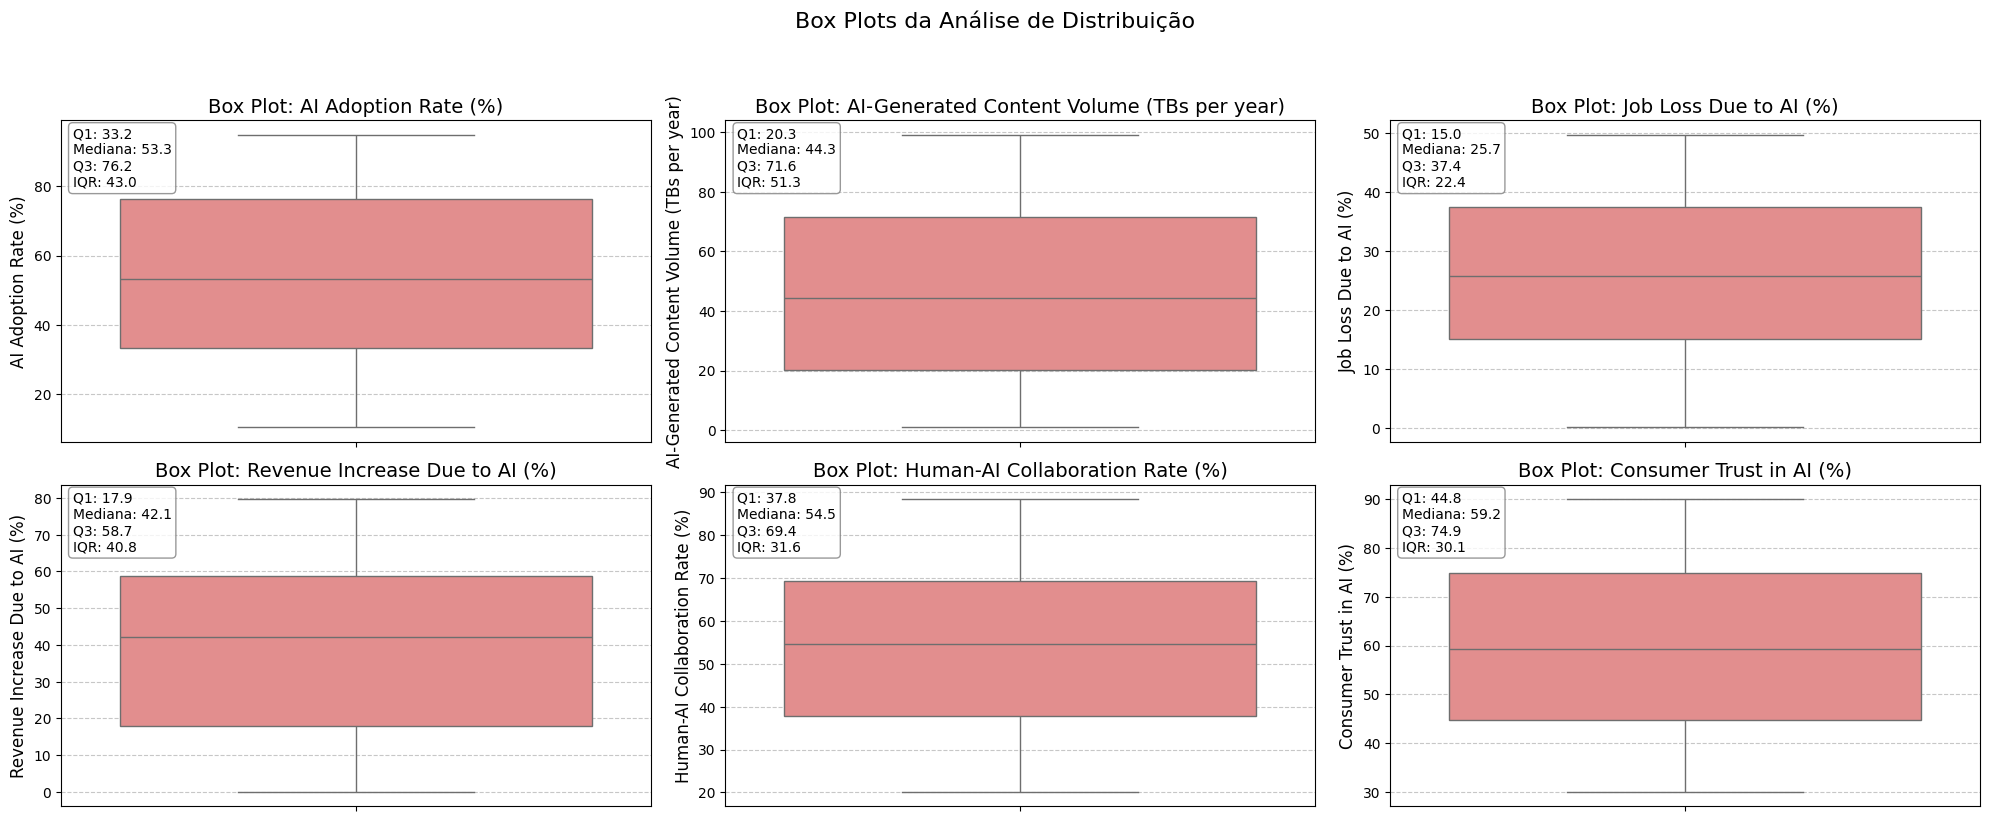
\includegraphics[width=1\textwidth]{boxplots.png}
        \caption{Boxplots}
    \end{figure}

    \item \textbf{Histogramas:}
    \begin{figure}[H]
        \centering
        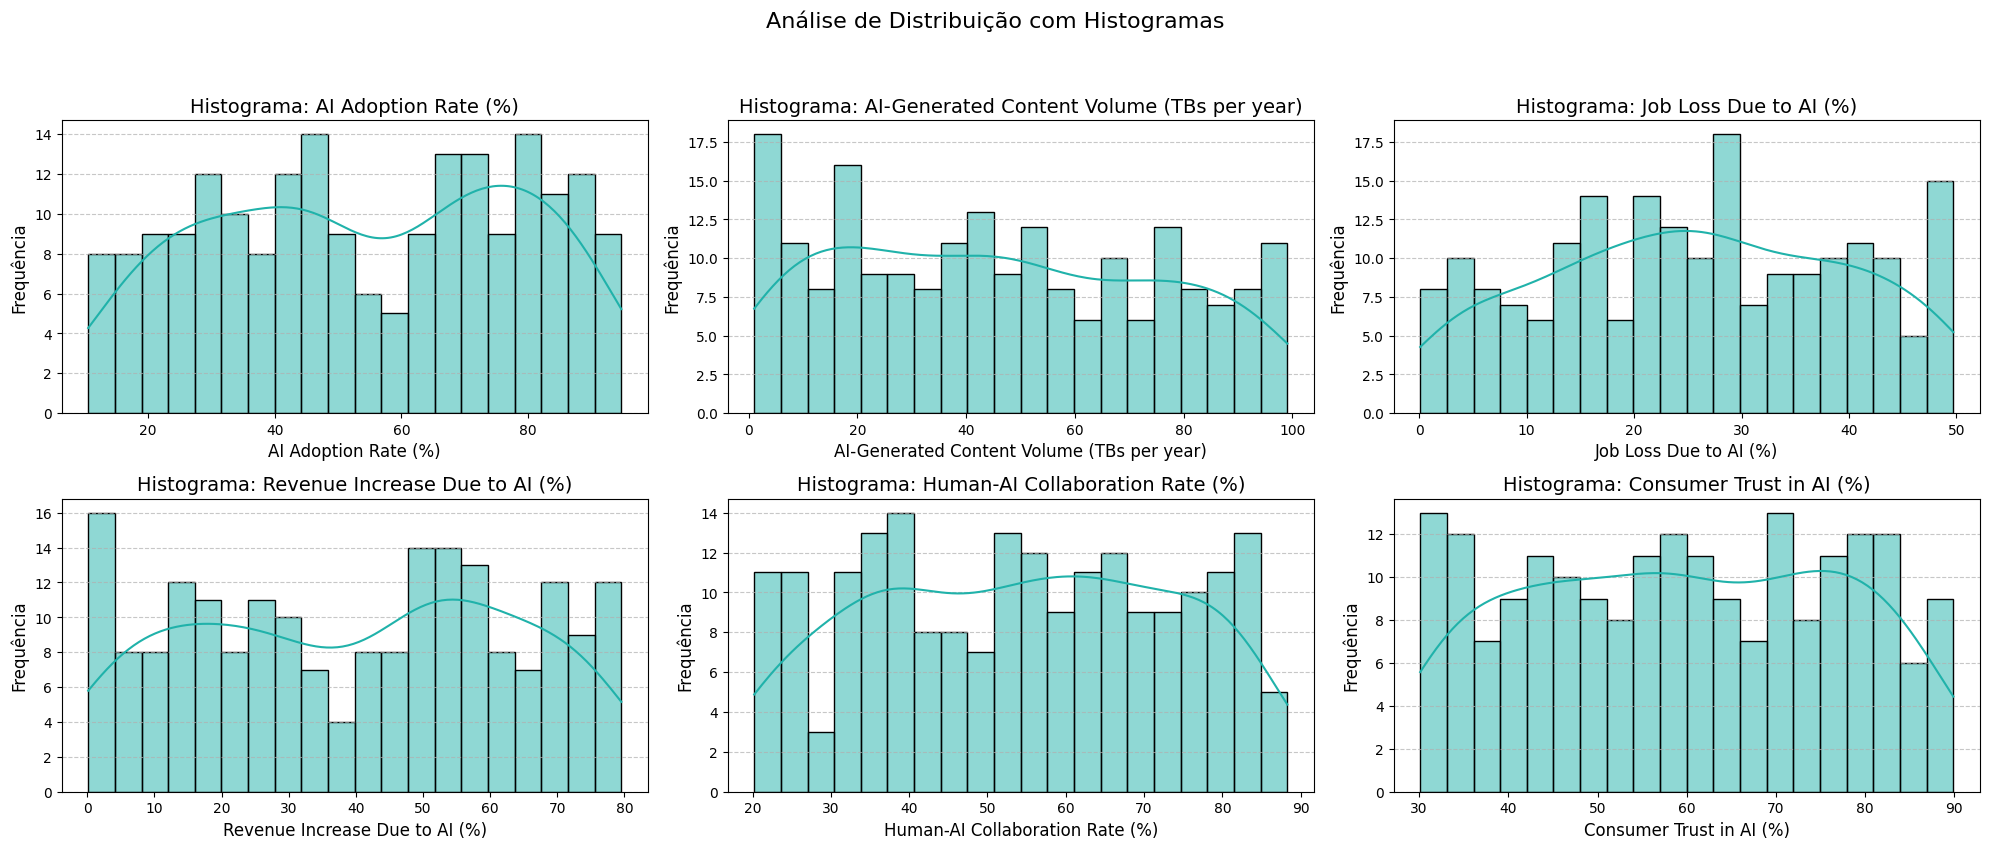
\includegraphics[width=1\textwidth]{histogramas.png}
        \caption{Histogramas}
    \end{figure}
\newpage
    \item \textbf{Scatter Plots:}
    \begin{figure}[H]
        \centering
        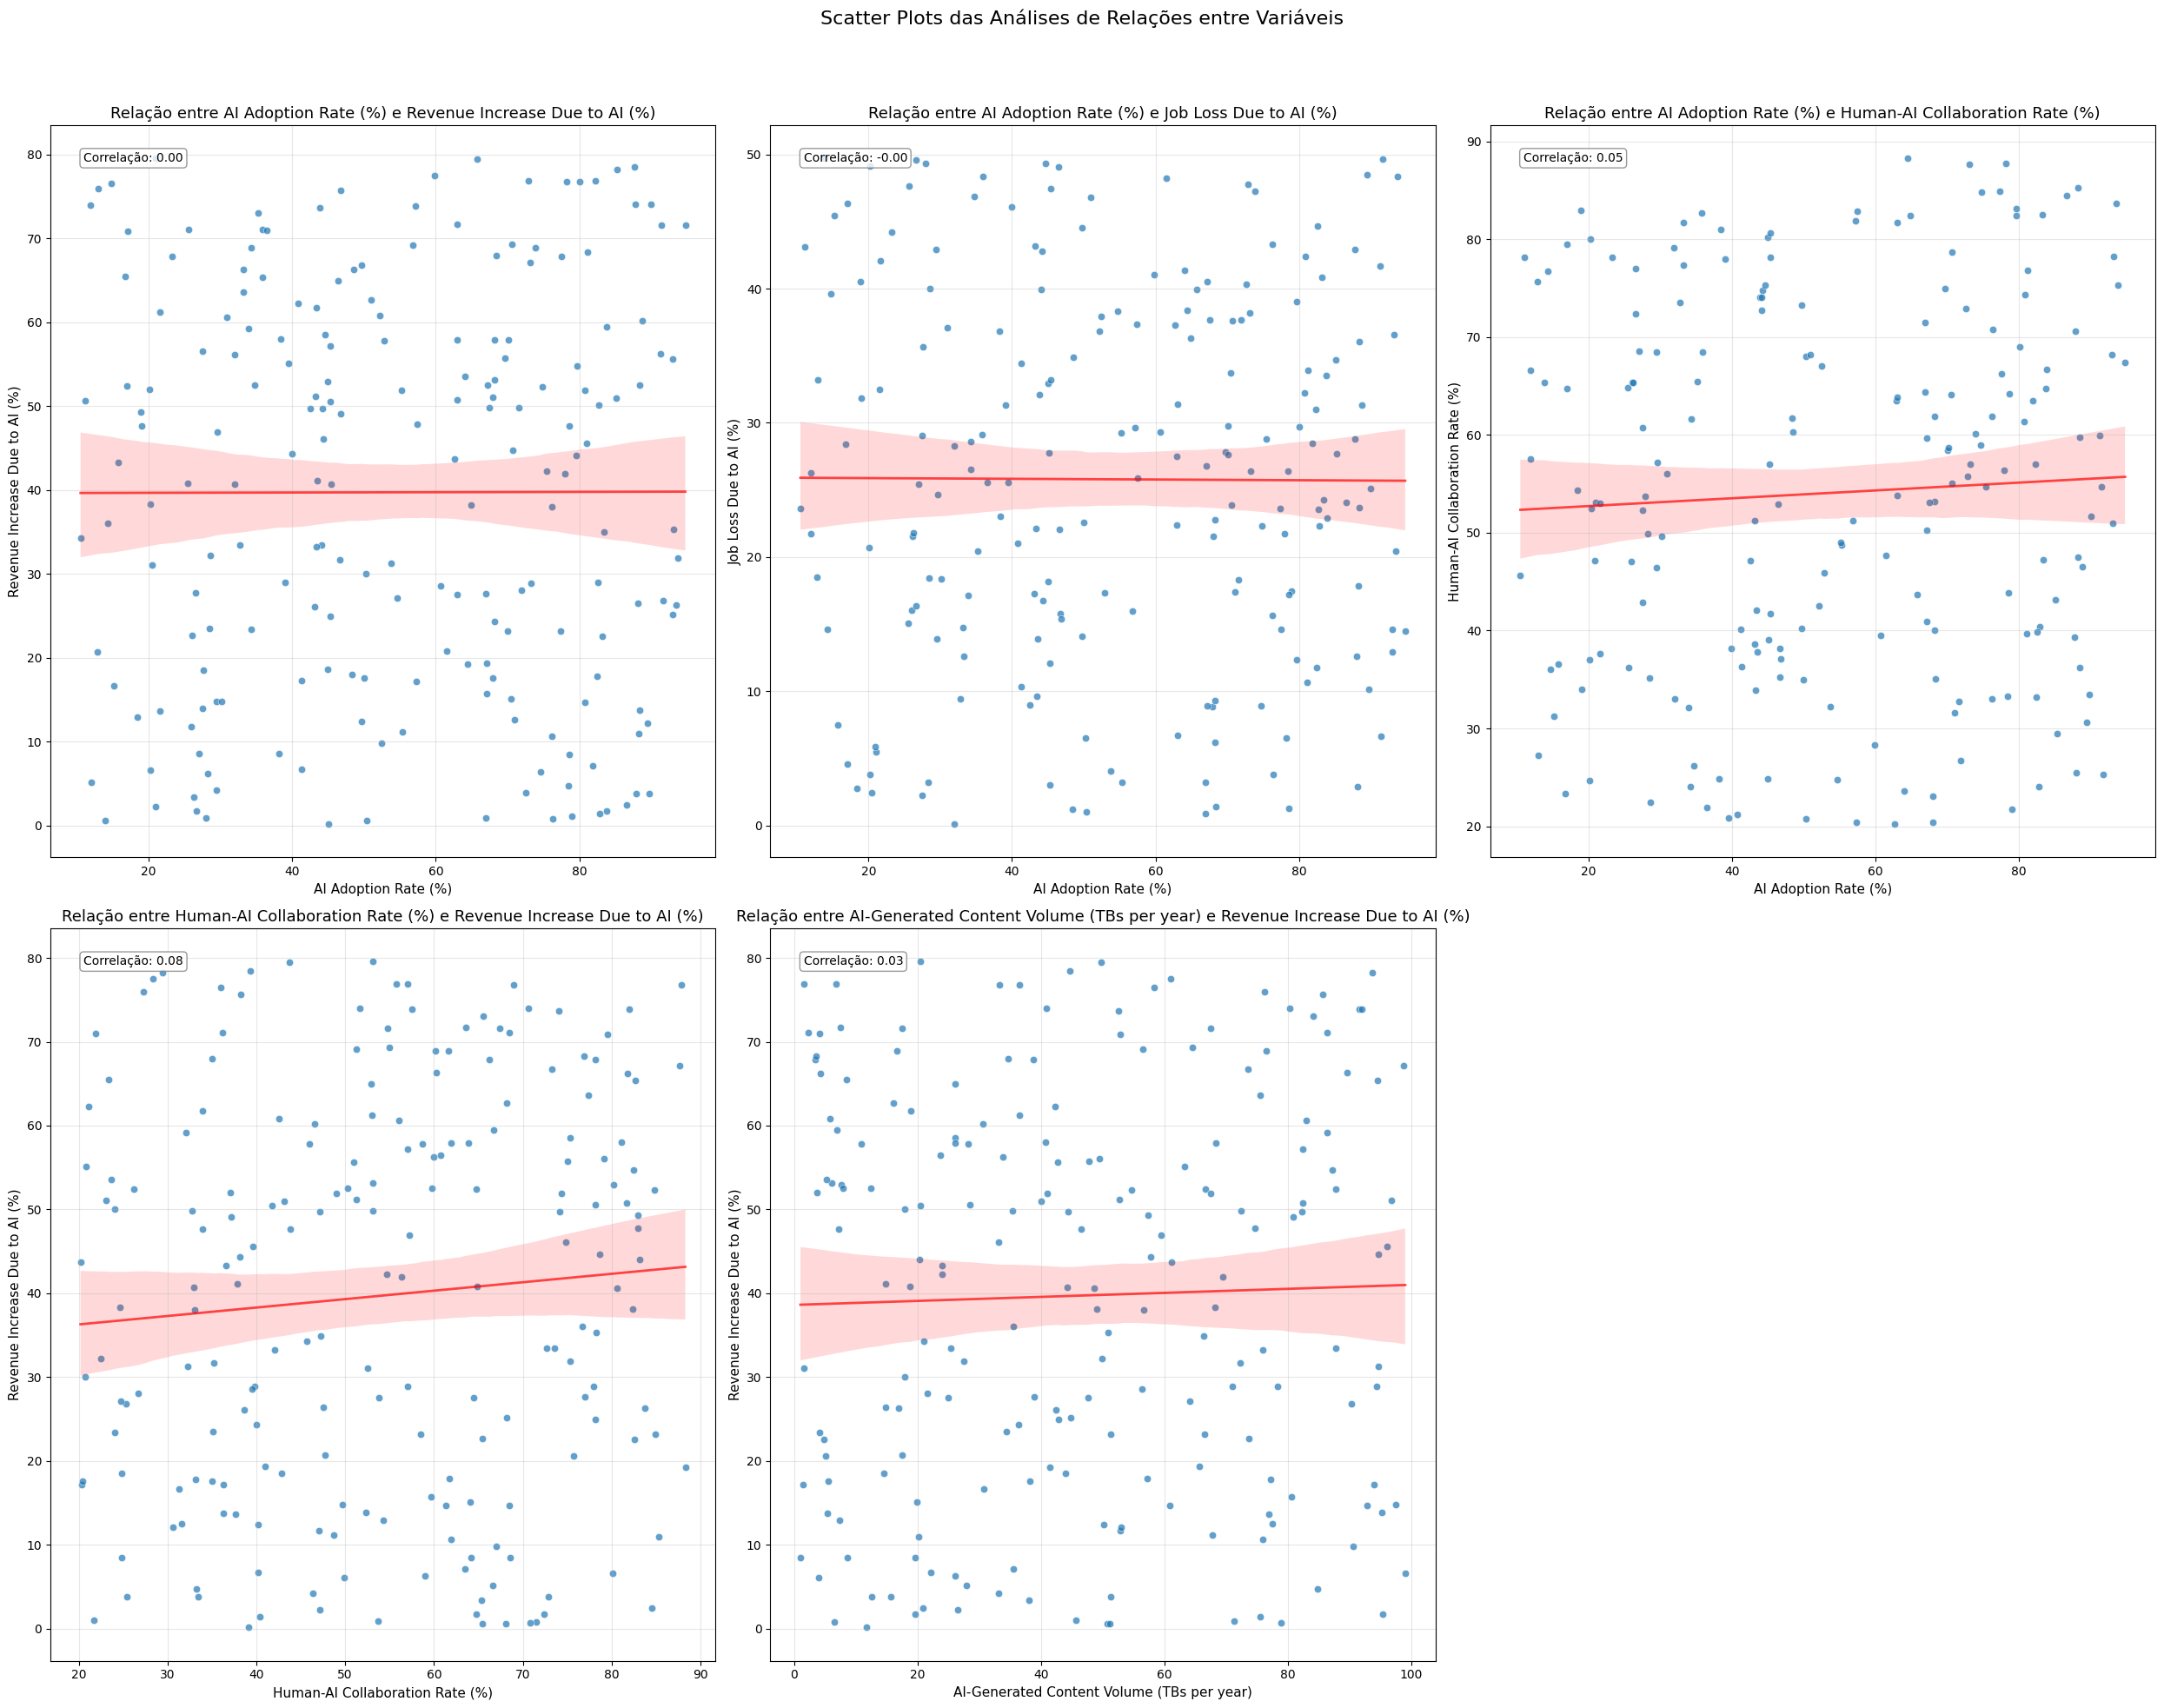
\includegraphics[width=1\textwidth]{scatter.png}
        \caption{Scatter Plots}
    \end{figure}
\newpage
    \item \textbf{Mapa de Calor:}
    \begin{figure}[H]
        \centering
        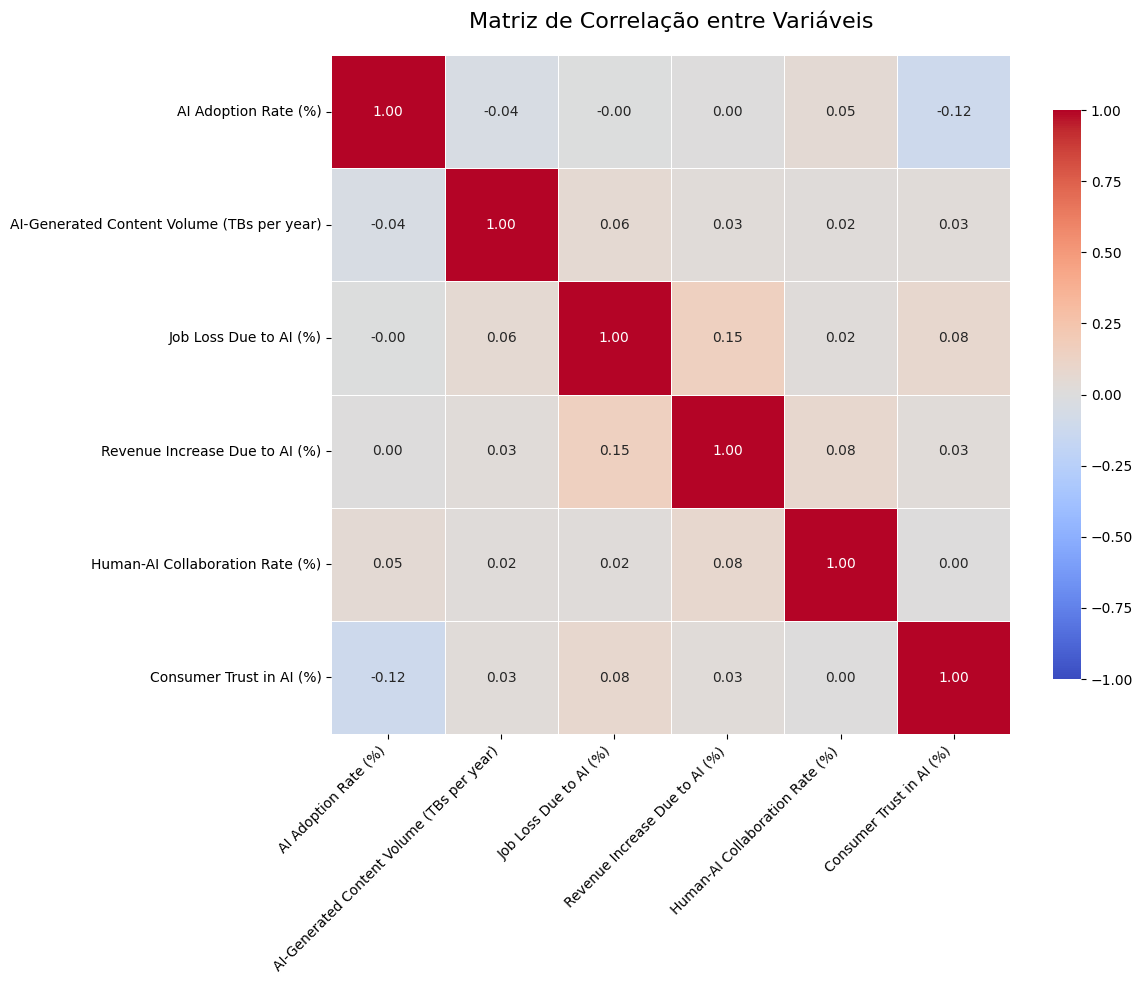
\includegraphics[width=1\textwidth]{heatmap.png}
        \caption{Mapa de calor}
    \end{figure}
\end{itemize}

\textbf{\textit{Interpretação}}: A análise dos dados foi realizada por meio de box plots, histogramas, scatter plots e mapa de calor com os seguintes destaques:

\begin{itemize}
  \item Os box plots revelaram grande variabilidade nas respostas, com medianas moderadas e nenhum outlier, o que indica diversidade nas percepções e impactos da IA.
  
  \item Os histogramas mostraram que algumas variáveis, como Receita e Colaboração, são distribuidas mais amplamente, enquanto Perda de Empregos e Confiança no Consumidor tendem a se concentrar em faixas específicas.
  
  \item As correlações entre Taxa de Adoção de IA, Receita, Perda de Empregos, Colaboração Humano-IA e Volume de Conteúdo foram muito baixas, indicando nenhuma relação forte.

  \item O mapa de calor reforça que não há relações lineares significativas entre as variáveis, sugerindo que os resultados podem estar sendo influênciados por outros fatores.
\end{itemize}

Os dados indicam que embora a IA esteja sendo adotada, seus efeitos sobre receita, empregos e colaboração ainda não seguem padrões claros ou previsíveis.

\subsection*{3.2 Normalização Padrão}

As variáveis \texttt{AI Adoption Rate (\%)},
\texttt{Revenue Increase Due to AI (\%)} e 
\texttt{AI-Generated Content Volume (TBs per year)} foram normalizadas usando a técnica de z-score:

\begin{equation}
z = \frac{x - \mu}{\sigma}
\end{equation}

\begin{itemize}
    \item \textbf{Amostra do dataframe normalizado:}
    \begin{table}[H]
    \centering
    \begin{adjustbox}{max width=\textwidth}
    \begin{tabular}{lrrrrrrr}
    \toprule
    Country & AI Adopt. & Revenue AI & Content (TB) & AI Adopt. (Z) & Revenue (Z) & Content (Z) \\
    \midrule
    South Korea & 44.29 & 46.12 & 33.09 & -0.4119 & 0.2686 & -0.4452 \\
    China       & 34.75 & 52.46 & 66.74 & -0.8058 & 0.5347 &  0.7087 \\
    USA         & 81.06 & 45.60 & 96.13 &  1.1064 & 0.2468 &  1.7166 \\
    France      & 85.24 & 78.24 & 93.76 &  1.2790 & 1.6165 &  1.6353 \\
    France      & 78.95 &  1.05 & 45.62 &  1.0192 & -1.6228 & -0.0155 \\
    USA         & 66.95 & 27.58 & 47.72 &  0.5237 & -0.5094 &  0.0565 \\
    Australia   & 68.23 & 53.13 &  6.14 &  0.5766 & 0.5628 & -1.3694 \\
    UK          & 91.27 & 56.26 & 33.87 &  1.5280 & 0.6941 & -0.4185 \\
    Canada      & 17.02 & 52.45 & 87.77 & -1.5379 & 0.5342 &  1.4299 \\
    China       & 25.50 & 40.81 & 18.74 & -1.1878 & 0.0458 & -0.9373 \\
    \bottomrule
    \end{tabular}
    \end{adjustbox}
    \caption{Primeiras 10 linhas do DataFrame com variáveis normalizadas}
    \end{table}
    \item \textbf{Resultados obtidos:}
    
        \begin{verbatim}
        Variável: AI Adoption Rate (%)
        Média original: 54.27
        Desvio padrão original: 24.22
        Média normalizada: -0.00000000
        Desvio padrão normalizado: 1.00000000
        --------------------------------------------------
        Variável: Revenue Increase Due to AI (%)
        Média original: 39.72
        Desvio padrão original: 23.83
        Média normalizada: 0.00000000
        Desvio padrão normalizado: 1.00000000
        --------------------------------------------------
        Variável: AI-Generated Content Volume (TBs per year)
        Média original: 46.07
        Desvio padrão original: 29.16
        Média normalizada: -0.00000000
        Desvio padrão normalizado: 1.00000000
        --------------------------------------------------
        \end{verbatim}
        
        \item \textbf{Visualização:}
        \begin{figure}[H]
        \centering
        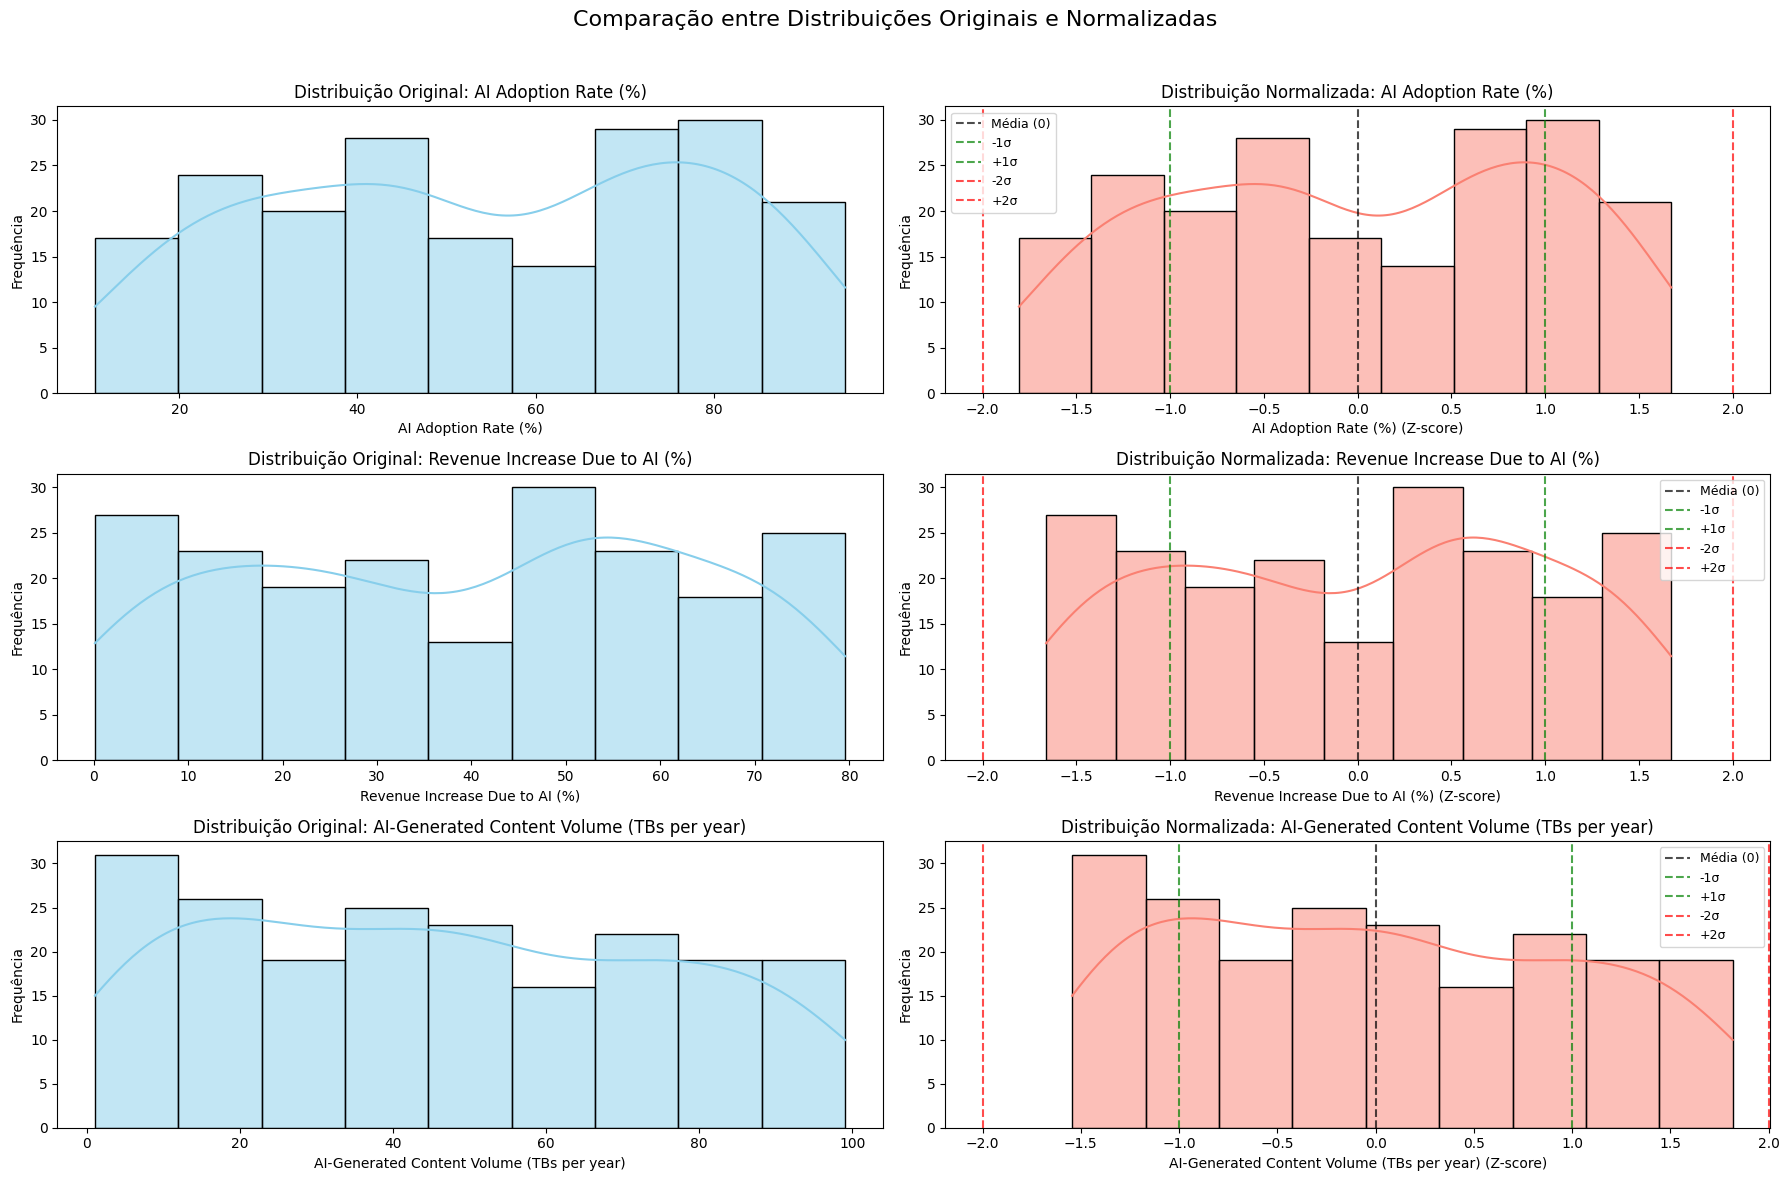
\includegraphics[width=1\textwidth]{normalpadrao.png}
        \caption{Distribuições originais x normalizadas}
        \end{figure}
    \item \textbf{\textit{Interpretação}}: Na saída é possível observar que que a média original da variável "AI Adoption Rate (\%)" foi de 54,27, com um desvio padrão de 24,22. Após a normalização, a média passou a ser praticamente zero e o desvio padrão exatamente um, indicando que a variável foi normalizada. O mesmo comportamento é observado para as outras duas variáveis analisadas, que foram "Revenue Increase Due to AI (\%)" que tinha uma média original de 39,72 e desvio de 23,83, enquanto "AI-Generated Content Volume (TBs per year)" possuía média 46,07 e desvio de 29,16.

    Além disso, no Dataframe após a normalização é possível observar como os valores foram redistribuídos em torno de zero. Por exemplo, os Estados Unidos apresentaram valores normalizados bem acima da média nas três métricas, indicando desempenho acima do esperado nessas dimensões. Já a China, apesar de uma adoção de IA abaixo da média, demonstrou aumento de receita e volume de conteúdo gerado acima da média, o que pode indicar um uso mais eficiente da tecnologia no país.
    
\end{itemize}

\subsection*{3.3 Distribuições Amostrais das Médias}

Seguindo o exemplo de distribuição amostral das médias apresentado em sala de aula, foram geradas distribuições amostrais para três variáveis: \texttt{AI Adoption Rate (\%)}, \texttt{Revenue Increase Due to AI (\%)} e \texttt{Job Loss Due to AI (\%)}. Para cada variável, foram realizadas 1500 amostragens com reposição, variando o tamanho da amostra entre 5, 15 e 30 observações.

\begin{itemize}
    \item \textbf{Resultados Obtidos:}
    \begin{verbatim}
    Variável: AI Adoption Rate (%)
    Média populacional: 54.27
    Desvio padrão populacional: 24.16
    --------------------------------------------------
    Tamanho da amostra: 5
    Média das médias amostrais: 54.50
    Erro padrão observado: 10.74
    Erro padrão teórico: 10.80
    ------------------------------
    Tamanho da amostra: 15
    Média das médias amostrais: 54.10
    Erro padrão observado: 6.30
    Erro padrão teórico: 6.24
    ------------------------------
    Tamanho da amostra: 30
    Média das médias amostrais: 54.47
    Erro padrão observado: 4.44
    Erro padrão teórico: 4.41
    ------------------------------

    Variável: Revenue Increase Due to AI (%)
    Média populacional: 39.72
    Desvio padrão populacional: 23.77
    --------------------------------------------------
    Tamanho da amostra: 5
    Média das médias amostrais: 39.95
    Erro padrão observado: 10.50
    Erro padrão teórico: 10.63
    ------------------------------
    Tamanho da amostra: 15
    Média das médias amostrais: 39.48
    Erro padrão observado: 6.08
    Erro padrão teórico: 6.14
    ------------------------------
    Tamanho da amostra: 30
    Média das médias amostrais: 39.87
    Erro padrão observado: 4.47
    Erro padrão teórico: 4.34
    ------------------------------

    Variável: Job Loss Due to AI (%)
    Média populacional: 25.79
    Desvio padrão populacional: 13.87
    --------------------------------------------------
    Tamanho da amostra: 5
    Média das médias amostrais: 25.47
    Erro padrão observado: 5.98
    Erro padrão teórico: 6.20
    ------------------------------
    Tamanho da amostra: 15
    Média das médias amostrais: 26.00
    Erro padrão observado: 3.48
    Erro padrão teórico: 3.58
    ------------------------------
    Tamanho da amostra: 30
    Média das médias amostrais: 25.71
    Erro padrão observado: 2.57
    Erro padrão teórico: 2.53
    ------------------------------
    \end{verbatim}
    
    \newpage
    \item \textbf{Visualização:}
    
    \begin{figure}[H]
    \centering
    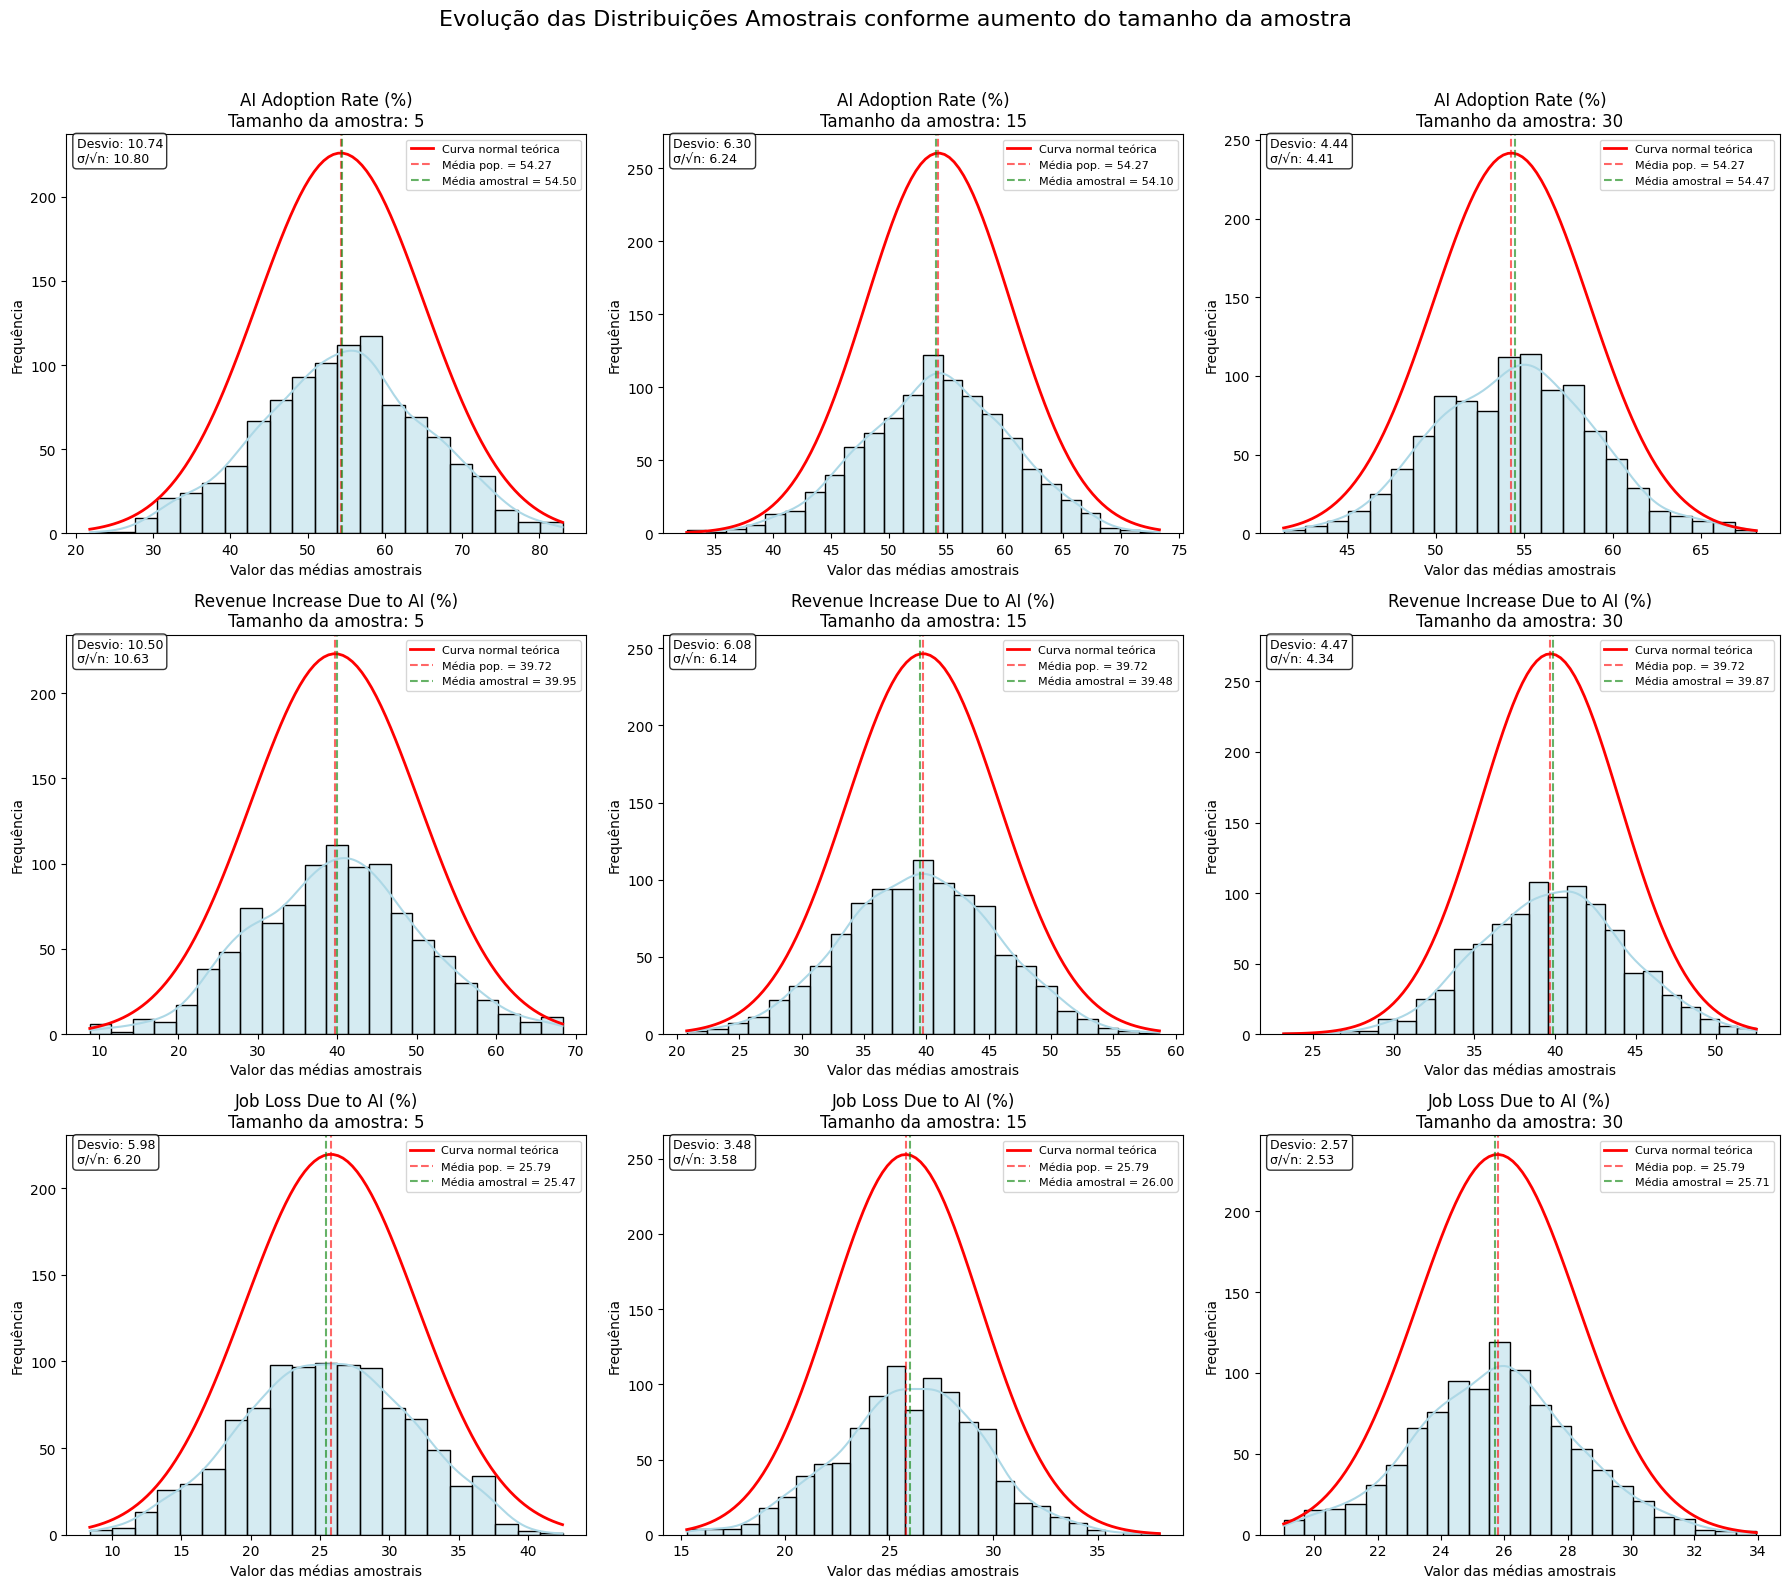
\includegraphics[width=1\textwidth]{distribuicoesamostrais.png}
    \caption{Relação das distribuições com o tamanho da amostra}
    \end{figure}

    \item \textbf{\textit{Interpretação}}: A análise das distribuições amostrais mostra que, conforme o tamanho da amostra aumenta, a média das médias amostrais se aproxima cada vez mais da média populacional — um resultado esperado segundo o Teorema Central do Limite. Além disso, o desvio padrão das médias amostrais diminui com o aumento de \( n \), o que significa que as estimativas se tornam mais precisas. 
    Por exemplo, para a variável \texttt{AI Adoption Rate (\%)}, o erro padrão passou de aproximadamente 10.74 para 4.44 ao aumentar o tamanho da amostra de 5 para 30.
    
\end{itemize}

\subsection*{3.4 Intervalos de Confiança}

Nesta etapa, foram calculados intervalos de confiança para a média populacional de três variáveis: \texttt{AI Adoption Rate (\%)}, \texttt{Revenue Increase Due to AI (\%)} e \texttt{Human-AI Collaboration Rate (\%)}. Os intervalos foram construídos com níveis de confiança de 90\% e 95\%, com base em uma amostra de tamanho 200 para cada variável.

\begin{itemize}
    \item \textbf{Resultados Obtidos:}
    \begin{verbatim}
    Variável: AI Adoption Rate (%)
    Tamanho da amostra: 200
    Média amostral: 54.27
    Desvio padrão amostral: 24.22
    --------------------------------------------------
    Intervalo de Confiança de 90%:
    IC = [51.44, 57.10]
    Margem de erro: ±2.83
    ------------------------------
    Intervalo de Confiança de 95%:
    IC = [50.89, 57.64]
    Margem de erro: ±3.38
    ------------------------------

    Variável: Revenue Increase Due to AI (%)
    Tamanho da amostra: 200
    Média amostral: 39.72
    Desvio padrão amostral: 23.83
    --------------------------------------------------
    Intervalo de Confiança de 90%:
    IC = [36.93, 42.50]
    Margem de erro: ±2.78
    ------------------------------
    Intervalo de Confiança de 95%:
    IC = [36.40, 43.04]
    Margem de erro: ±3.32
    ------------------------------

    Variável: Human-AI Collaboration Rate (%)
    Tamanho da amostra: 200
    Média amostral: 54.10
    Desvio padrão amostral: 19.25
    --------------------------------------------------
    Intervalo de Confiança de 90%:
    IC = [51.85, 56.35]
    Margem de erro: ±2.25
    ------------------------------
    Intervalo de Confiança de 95%:
    IC = [51.42, 56.79]
    Margem de erro: ±2.68
    ------------------------------
    \end{verbatim}

    \item \textbf{Visualização:}
    
    \begin{figure}[H]
    \centering
    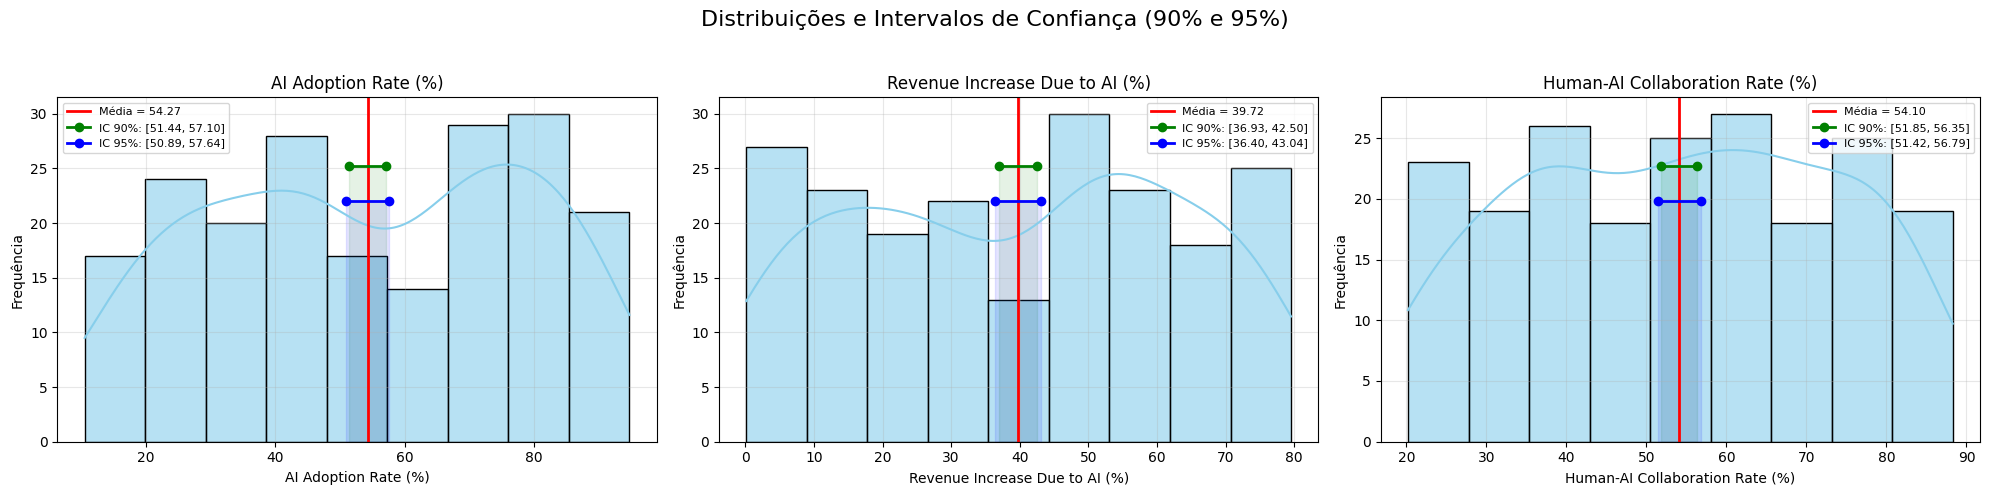
\includegraphics[width=1\textwidth]{intervaloconfianca.png}
    \caption{Intervalos de confiança de 90\% e 95\% para as três variáveis analisadas}
    \end{figure}

    \item \textbf{\textit{Interpretação}}: Os intervalos de confiança indicam que as estimativas de média para as três variáveis analisadas são confiáveis, com margens de erro relativamente pequenas considerando o tamanho amostral de 200. 
    
    Por exemplo, para a variável \texttt{Human-AI Collaboration Rate (\%)}, com 95\% de confiança, espera-se que a verdadeira média populacional esteja entre 51.42\% e 56.79\%, refletindo um nível consistente de interação entre humanos e IA nos países analisados.
    
\end{itemize}

\section*{4. CONCLUSÃO}

Com base nas análises realizadas, foi possível compreender com maior clareza o comportamento das variáveis relacionadas ao impacto da Inteligência Artificial em diferentes setores e países. A simulação de distribuições amostrais evidenciou o efeito do Teorema Central do Limite, mostrando que médias amostrais se aproximam da média populacional com o aumento do tamanho da amostra, além da redução do erro padrão. Já os intervalos de confiança permitiram estimar com precisão as médias populacionais das variáveis analisadas.

Destaca-se, por exemplo, que a taxa média de adoção de IA está em torno de 54\%, enquanto o aumento médio de receita associado ao uso de IA é de aproximadamente 40\%. Esses dados sugerem uma relação positiva entre a adoção de IA e o desempenho financeiro das organizações. Além disso, a colaboração entre humanos e IA apresentou valores médios consistentes, indicando que a integração entre tecnologia e capital humano está em processo de consolidação, o que reflete as mudanças no mundo que ocorreram após a popularização dessa tecnologia.

Portanto, os resultados obtidos servem de base para futuras decisões governamentais e acadêmicas sobre regulação da IA, em contextos de rápida transformação tecnológica como é possível ver atualmente.

\section*{5. REFERÊNCIAS}

\begin{itemize}
    \item Material didático da disciplina de Estatística e Probabilidade, fornecido pelo professor.
    \item SOUNDANKAR, Atharva. \textit{Impact of AI on Digital Media (2020–2025)}. Kaggle, 2023. Disponível em: \url{https://www.kaggle.com/datasets/atharvasoundankar/impact-of-ai-on-digital-media-2020-2025}.
\end{itemize}

\end{document}